\chapter{Asking Dubai Moguls How They Got Rich!}

This chapter follows a School of Hard Knocks interview, curated by LazyingArt LLC, and it is best read as a guided sequence of business constructions rather than as a pile of disconnected success stories. We begin with spectacle, but almost immediately the lecture starts converting spectacle into structure: first hardship and sales, then speed of scale, then the social mechanics of business formation, and finally a stage rule for concentration, diversification, and reinvestment.

\section{Cold Open: Dubai, Scale, and the Teaser Splice}

The lecture opens by spending surprise before explanation. We are shown fragments of later claims: a Lamborghini, a blockchain company, one-year earnings in the eight figures, a billion-dollar company, and a net-worth-like figure near three hundred million dollars. These numbers should not be fused into one stable balance sheet. They are a teaser splice, not yet a single argument. Their job is to say that the episode will operate at visible scale.

Only after that splice does the host reset the frame. We are in Dubai, and the city is treated as a field site in which wealth is displayed publicly enough that one may ask, in the open, how it was built. This reset matters. The lecture does not want us to stare at the car. It wants us to move from the car to the mechanism:
\begin{equation}
\text{visible luxury}
\to
\text{question}
\to
\text{business mechanism}.
\end{equation}
That is the governing rhythm of the chapter.

\section{The First Lamborghini: Duration, Hardship, and Control}

The first sustained case is the finance entrepreneur who steps out of a Lamborghini. The lecturer does not begin with philosophy. He begins with duration and scale,
\begin{align}
t_{\text{James}} &\approx 8\ \text{years}, \\
Y_{\text{James}}^{\text{turnover}} &\approx \$12\,\text{million},
\end{align}
and only after that does he pull the story backward into difficulty:
\begin{equation}
R_{\text{rent}} \approx \$1{,}300.
\end{equation}
That rent threshold is not a decorative detail. It is the lecture's first serious benchmark. There was a time, we are told, when even that amount could not be covered, and wedding jewelry had to be sold to pay rent. The chapter should preserve this ordering. First scale, then contrast, then the question of what changed.

The answer, at first, is inward rather than technical. The speaker says the turning point was partly the refusal to accept the social verdict attached to not finishing school. He describes himself as the black sheep of the family and recasts that status as fuel. But the lecture does not stay long in that motivational register. It quickly narrows to a sharper business point: a founder must have ``full control over the money.'' Here we should not pretend the lecture has given us a formal accounting identity. What it gives instead is a doctrine of operational visibility. One must know where money comes from, where it goes, and who actually controls the channels through which it moves.

Only after that does the host ask the natural next question. If the business is real, if the hardship is real, and if the money is now substantial, how was the commercial engine actually run?

\section{Rejection, Yes-Ladders, and the Arithmetic of Scarcity}

Now the lecture tightens. The speaker says he used to do door-to-door sales, and from that world he extracts the clearest piece of explicit arithmetic in the entire chapter:
\begin{equation}
N_{\text{doors}} = 100.
\end{equation}
The point is not simply persistence. The point is that repeated rejection is treated as data. Each no is not final defeat; it is a local measurement that modifies the next attempt. The lecture's sequence may be written in compact form as
\begin{equation}
\text{rejection} \to \text{learning} \to \text{adjusted question} \to \text{higher chance of yes}.
\end{equation}
At this stage the lecture is still close to the ground. We are not given a universal theory of persuasion. We are given field craft.

\subsection{Question \& Answer}

What, then, does it mean to get to yes faster? The speaker's answer is very concrete. Instead of opening with the real demand, we begin by collecting easy affirmations:
\begin{equation}
n_{\text{ask}} \approx 4\text{--}5,
\qquad
\text{yes} \to \text{yes} \to \text{yes} \to \text{ask}.
\end{equation}
The transcript even provides a worked example. The host asks:
\begin{align}
Q_1 &: \text{Are you in Dubai?} & A_1 &= \text{yes}, \\
Q_2 &: \text{Do you like the weather here?} & A_2 &= \text{yes}, \\
Q_3 &: \text{Do you like the vibe here?} & A_3 &= \text{yes}, \\
Q_4 &: \text{Would you like to own property here one day?} & A_4 &= \text{soft yes}.
\end{align}
The lecture's claim is that once several small agreements are in place, the actual ask arrives in a softened environment. In compact notation,
\begin{equation}
P(\text{yes on ask }4\text{ or }5)\ \text{rises after repeated local yeses}.
\end{equation}
This is not a measured theorem. It is a commercial heuristic. But it is precisely the kind of heuristic the lecture wants to preserve: not merely ``be confident,'' but ask in a sequence that structures the answer.

\begin{figure}[h]
\centering
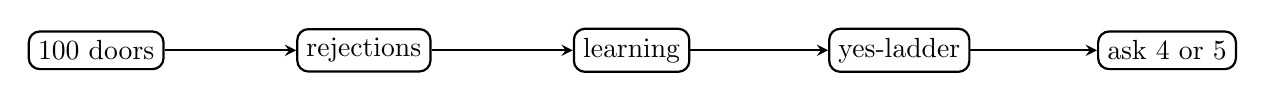
\begin{tikzpicture}[>=stealth, thick]
\node[draw, rectangle, rounded corners] (a) at (0,0) {\(100\) doors};
\node[draw, rectangle, rounded corners] (b) at (3.4,0) {rejections};
\node[draw, rectangle, rounded corners] (c) at (6.8,0) {learning};
\node[draw, rectangle, rounded corners] (d) at (10.2,0) {yes-ladder};
\node[draw, rectangle, rounded corners] (e) at (13.6,0) {ask \(4\) or \(5\)};
\draw[->] (a) -- (b);
\draw[->] (b) -- (c);
\draw[->] (c) -- (d);
\draw[->] (d) -- (e);
\end{tikzpicture}
\caption{Transcript-based reconstruction of the first speaker's sales mechanism.}
\end{figure}

The lecture now broadens from sales to austerity. The same speaker returns to the broke phase and insists that the middle class often weakens itself through constant leakage: subscriptions, small comforts, debt, and premature rewards. The transcript is garbled at the level of tiny monthly figures, so we should resist the temptation to invent a clean expenditure model. The reliable point is more structural:
\begin{equation}
\text{scarcity} \to \text{cut leakage} \to \text{save} \to \text{invest} \to \text{reward later}.
\end{equation}
Then comes the last movement of this first case. If one has an idea, one should execute it. Advice from people without business experience is not treated as neutral information; it is treated as drag. The first interview therefore closes by tying together hardship, control of money, sales sequence, and disciplined execution. The host then briefly recaps the lesson outside the luxury hotel: a man who once struggled to pay roughly a thousand dollars in rent is now making more than ten million dollars a year. The recap matters because it turns anecdote into scale contrast before the lecture pivots again.

\section{Fast Unicorns, Timing, and the Web3 Friction Thesis}

The second major case changes the tempo immediately. We go from eight years of compounding struggle to a company that reaches unicorn scale in less than a year:
\begin{align}
\Delta t_{\text{raise}} &\approx 11\ \text{months}, \\
M_{\text{raised}} &> \$100\,\text{million}, \\
V_{\text{company}} &\approx \$1.5\,\text{billion}.
\end{align}
This is the lecture's cleanest capital-formation example. The company is said to have started in April 2021. In roughly eleven months it raised more than one hundred million dollars and reached a valuation of one and a half billion. One simple derived quantity helps us feel the speed:
\begin{equation}
\frac{M_{\text{raised}}}{\Delta t_{\text{raise}}}
>
\frac{\$100\,\text{million}}{11\ \text{months}}
\approx
\$9.1\,\text{million per month}.
\end{equation}
The lecture itself does not compute the ratio, but the arithmetic is faithful to the transcript and clarifies the claim.

\subsection{Question \& Answer}

Can somebody get rich quickly in such a world? The answer given in the interview is much more disciplined than the phrase sounds. It is not simply ``yes, because crypto.'' It is: yes, if one is in the right place at the right time, where place means industry as much as geography. The speaker compresses this into a historical ladder,
\begin{equation}
1990\text{s} \to \text{internet},
\qquad
2010\text{s} \to \text{social media},
\qquad
2020\text{s} \to \text{AI / blockchain / Web3}.
\end{equation}
So ``getting rich quick'' is not, in the lecture's own reasoning, magic. It is temporal matching. It is choosing a sector whose curve has not yet flattened.

Now the lecture inserts an important motivational beat that the first draft handled too lightly. The blockchain founder says he came from a humble family, that even a Starbucks coffee was once a luxury, and that being broke was an advantage because it taught the importance of money. Only after that background does the host ask the next sharp question: what do banks not want people to know?

The answer is a rhetorical contrast rather than a theorem of finance. Banks make money on our money; crypto, by contrast, is presented as a system in which our own money can compound more directly. The lecture expresses this not as balance-sheet algebra but as a friction claim:
\begin{align}
c_{\text{crypto}}(\$10\,\text{million}) &\approx \$1, \\
T_{\text{crypto exit}}(\$15\,\text{million}) &\approx 1\ \text{minute}.
\end{align}
These statements should remain attributed. They are part of the interview's doctrine, not general financial law.

The same doctrine is immediately extended into a social claim: Web3 is said to be a ladder along which poor become middle class, middle class become upper middle class, and upper middle class become rich. Then the ladder is made temporal again through the language of the 2021 bull run and the predicted 2025 bull run. We should preserve this movement, but preserve it cautiously. The lecture is most solid here when it speaks about timing and transfer friction, less solid when it predicts the full architecture of class mobility.

A sponsor segment breaks the flow at this exact point. It is worth preserving one sentence of its logic: the host says that rapid fundraising on this scale depends on communication as much as on mere ambition. That observation forms a natural bridge into the next interview, where communication and relationship become the main subject.

\section{Non-Transactional Networking, Execution, and Collision Hours}

After the sponsor hinge the lecture changes register. We move from timing and capital formation to human method. A venture-capital and tech operator, who says he has been broke many times, is asked about the richest people he has met. That question opens the door to the strongest relational doctrine in the chapter: if one wants to talk to billionaires, one should not begin by talking about work. One should begin by knowing them as people.

The local mechanism can be written compactly as
\begin{equation}
\text{human conversation}
\to
\text{shared affinity}
\to
\text{trust}
\to
\text{business opportunity}.
\end{equation}
The lecture insists that the best businesses are often born out of conversations that were not initially about business at all. The human relationship comes first. Only later does the transaction become possible.

\subsection{Question \& Answer}

Why should some of the best businesses begin in conversations that are not about business? Because, the speaker says, people usually damage the situation by entering with a desired outcome already loaded into the exchange. They are trying to get something before they have become knowable. The lecture therefore inverts the usual strategy. Do not begin with extraction. Begin with personhood. If the interaction becomes genuinely human, business may arise later as a byproduct rather than as a demand.

At this precise point the lecture pivots, quite beautifully, from relationship to execution. The speaker invokes the Snuggie as a canonical example:
\begin{equation}
S_{\text{Snuggie}} \approx \$100\,\text{million}.
\end{equation}
A blanket with sleeves is treated as a bad idea, yet one that was executed so effectively that it generated enormous sales. From this the speaker derives one of the cleanest inequalities in the lecture:
\begin{equation}
\text{bad idea executed well}
\;>\;
\text{great idea executed poorly}.
\end{equation}
This is not a general theorem of economics. It is a rule of commercial emphasis. The lecture wants us to stop worshiping idea quality in isolation.

The sequence does not stop there. The same speaker then turns against shyness. He says he began as a programmer, comfortable behind a screen, but that such comfort becomes a ceiling if one wants to build at scale. One must learn to run one's mouth, to meet people, to stand in lines, to pull tables together, to place coffees on the table, and to let conversations happen. This is where Tony Hsieh's language of ``Collision Hours'' becomes central. Creation does not arrive purely from solitary brilliance. It often arrives from designed contact.

\begin{figure}[h]
\centering
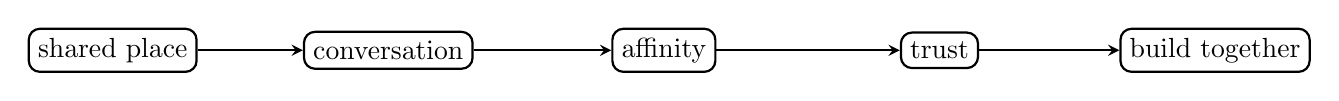
\begin{tikzpicture}[>=stealth, thick]
\node[draw, rectangle, rounded corners] (a) at (0,0) {shared place};
\node[draw, rectangle, rounded corners] (b) at (3.5,0) {conversation};
\node[draw, rectangle, rounded corners] (c) at (7,0) {affinity};
\node[draw, rectangle, rounded corners] (d) at (10.5,0) {trust};
\node[draw, rectangle, rounded corners] (e) at (14,0) {build together};
\draw[->] (a) -- (b);
\draw[->] (b) -- (c);
\draw[->] (c) -- (d);
\draw[->] (d) -- (e);
\end{tikzpicture}
\caption{Transcript-based reconstruction of the lecture's non-transactional networking sequence.}
\end{figure}

\section{Scale, Go-to-Market, and Building for \(t+5\)}

Only after the social mechanism is established does the host return to explicit business scale. He reminds the speaker of the claim that he made more than fifty million dollars in a year and asks how one moves from seven figures to eight. This transition should be preserved because it is one of the lecture's strongest narrative moves: first relationships, then the economic form that can actually scale.

The answer begins with the difference between digital and physical goods:
\begin{equation}
MC_{\text{digital}} \ll MC_{\text{physical}},
\qquad
\text{go-to-market reach} \to \text{global market}.
\end{equation}
When the product is software, each new unit is not constrained by the material burdens of ordinary production. That does not remove difficulty; it relocates it. The bottleneck shifts from manufacturing to distribution. So the lecture moves naturally to go-to-market strategy: define the product, identify the problem, find the people who want the solution, and use the internet to scale the match.

\subsection{Question \& Answer}

How do we choose a sector before the market has fully arrived? The lecture answers by turning its gaze forward. We are told to imagine the world five years from now and build for that world today:
\begin{equation}
\text{build at } t
\text{ for the world at } t+5.
\end{equation}
This is perhaps the most structurally useful formula in the chapter. It translates speculation into method. We do not merely chase what is already hot. We ask what the future state will require, and then we build inside the enabling layer that future depends upon.

The lecture's examples matter because they show how the speaker thinks. He does not say only ``AI.'' He says AI and automation, but also batteries, synthetic data, machine production, and AI-avatar content systems. These are peripheral systems, or supporting systems, or second-order systems. In other words, he is not only asking what the future object is; he is asking what machinery the future object needs in order to exist.

\begin{figure}[h]
\centering
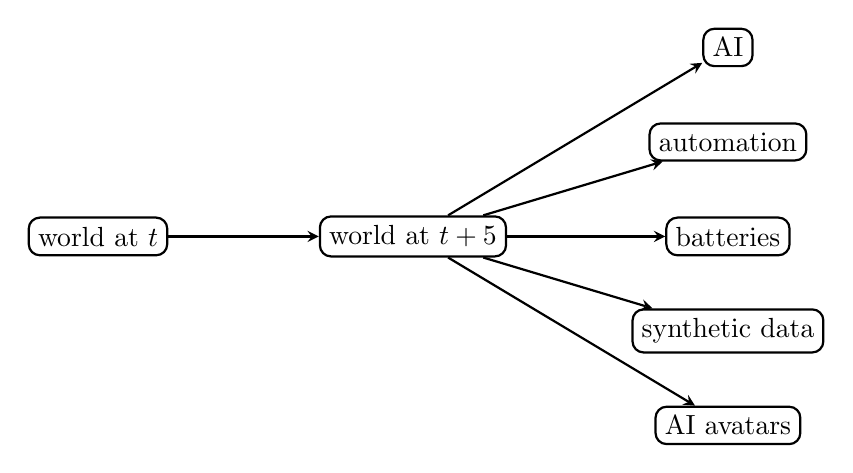
\begin{tikzpicture}[>=stealth, thick]
\node[draw, rectangle, rounded corners] (a) at (0,0) {world at \(t\)};
\node[draw, rectangle, rounded corners] (b) at (4,0) {world at \(t+5\)};
\node[draw, rectangle, rounded corners] (c1) at (8,2.4) {AI};
\node[draw, rectangle, rounded corners] (c2) at (8,1.2) {automation};
\node[draw, rectangle, rounded corners] (c3) at (8,0) {batteries};
\node[draw, rectangle, rounded corners] (c4) at (8,-1.2) {synthetic data};
\node[draw, rectangle, rounded corners] (c5) at (8,-2.4) {AI avatars};
\draw[->] (a) -- (b);
\draw[->] (b) -- (c1);
\draw[->] (b) -- (c2);
\draw[->] (b) -- (c3);
\draw[->] (b) -- (c4);
\draw[->] (b) -- (c5);
\end{tikzpicture}
\caption{Transcript-based reconstruction of the lecture's five-year forecasting rule.}
\end{figure}

The lecture then corrects any tendency toward glamour. The speaker says that mortgage technology, precisely because it sounds boring, is among the best businesses to own. This correction is important. The future-facing imagination of the lecture is not there to flatter fashionable language. It is there to teach sector selection under uncertainty.

\section{The Final Rolls-Royce: Concentration, Diversification, and the Return of Knowledge}

The final interview does not merely repeat the earlier blockchain case. It closes the chapter by changing the theory of capital. We are again given substantial numbers,
\begin{align}
Y_{\text{personal,last year}} &\approx \$100\,\text{million}, \\
W_{\text{net}} &\approx \$300\,\text{million},
\end{align}
and we should again quietly correct the host's mishearing of ``hundred billion'' to ``hundred million.'' But the real contribution of this case is not the amount. It is the stage rule that follows:
\begin{equation}
K_{\text{early}} \to \text{all-in concentration},
\qquad
K_{\text{late}} \to \text{diversification}.
\end{equation}
If one has no money, one must go all in on the idea. Once money exists, balance becomes essential.

\subsection{Question \& Answer}

When should we be concentrated, and when should we become balanced? The lecture answers without embarrassment. Early on, obsession is not merely tolerated; it is required. The founder speaks of relentless effort, of not giving up even when everyone leaves, of acting with a kind of madness while the first large breakthrough is still unfinished. That is the concentration phase. Later, once wealth has been built, the correct posture changes. Then one must diversify, refuse overexposure, and preserve what has been created.

The lecture then turns from capital allocation to specific investment advice. The founder says that for 2025 the best investment is Solana, described as faster, cheaper, and more scalable than its rivals. When asked about Bitcoin, however, he does not dismiss it. He places it in a different position: Bitcoin is where one puts most of the money, and then one places some capital elsewhere. In cautious reconstructed form, the portfolio rule is
\begin{equation}
W = W_{\text{BTC}} + W_{\text{SOL}} + W_{\text{other}},
\qquad
W_{\text{BTC}} \text{ largest}.
\end{equation}
We should be careful here. The blockchain comparison is technically compressed in the interview, and we should not pretend it has become a rigorous architecture lesson. But the allocation logic is clear enough: one core position, then secondary bets.

Next comes another important motivational beat. The founder says he has met many billionaires, that he grew up in Australia after being born in Lithuania, and that entrepreneurship is above all a matter of non-complacency and team quality. This is not a small addendum. The lecture wants to end by shifting the source of scale away from the isolated heroic self:
\begin{equation}
\text{talent} + \text{team} + \text{shareholder alignment} \to \text{larger enterprise}.
\end{equation}
``One person is nothing,'' he says in effect; people take us where money alone cannot.

Finally the biography turns once more toward loss and recovery. The founder says he came from no wealth, lived through the dot-com bubble, lost everything, learned from it, and later built again. The exact company names in the poker anecdote are unstable in the transcript, but the structural sequence is not:
\begin{equation}
\text{loss} \to \text{knowledge} \to \text{new construction} \to \text{new wealth}.
\end{equation}
And so the lecture closes not with consumption but with investment. Trust oneself, do what one loves, and invest in health, mind, business, markets, and people. The final claim is that life becomes interesting not when money is merely stored, but when it is repeatedly turned back into capacity.

\section{Summary}

The lecture begins with the sight of wealth and ends with a grammar for building it. First, hardship gives us a threshold against which later success becomes measurable. Second, sales is treated as a sequence of experiments, in which repeated no's become information and repeated yeses prepare the actual ask. Third, rapid scale is tied to timing, to capital access, and to sectors whose curves are still rising. Fourth, business opportunity emerges most powerfully from relationships that begin as human rather than transactional. Fifth, technology matters because it changes the geometry of replication and lets us build now for a world that is not yet fully here. Finally, the lecture ends with a stage rule: concentrate while building, diversify after scale, and keep translating loss into knowledge and knowledge into renewed enterprise.

In that sense Dubai is not the content of the lecture. It is the stage on which the deeper structure becomes visible. Wealth appears at the end as the car, the hotel, and the number. But the real mathematics of the chapter lies underneath: thresholds, sequences, timing, friction, scale, and the change of rule that comes when a founder moves from scarcity to abundance.